\documentclass[11pt, reqno]{amsart}
%\documentclass[12pt,twoside]{report}  % For two-sided numbering
\usepackage{fullpage}
\usepackage{amssymb,latexsym}
\usepackage{amsthm}
\usepackage{amsmath}
\usepackage{graphicx}
\usepackage{mathrsfs}
\usepackage{multirow}
%\usepackage{algpseudocode}
%\usepackage{program}
%\usepackage{algorithm}
%\usepackage{algorithm2e}
%\usepackage{algorithmicx}
%\usepackage{algorithm}
%\usepackage[noend]{algpseudocode}
\usepackage{bm}
\usepackage{enumerate,color,mathrsfs,epstopdf}
\usepackage{setspace}
\usepackage{url}
\usepackage{scalerel}
\usepackage{dsfont}
\usepackage{caption}
\usepackage{subcaption}

\usepackage{hyperref}
\hypersetup{
    colorlinks=true,
    linkcolor=blue,
    filecolor=magenta,      
    urlcolor=cyan,
}

\usepackage{algorithmic, algorithm2e, float} % all packages used for algorithm pseudocode
\usepackage[ruled,vlined,algo2e,linesnumbered]{algorithm2e}

%\alglanguage{pseudocode}

\setlength{\footskip}{50pt}


%\pagenumbering{gobble}


%%%%%%%%%%%%%%%% MACROS GO HERE %%%%%%%%%%%%%%%%%%%%%%%


\theoremstyle{plain}
\newtheorem{theorem}{Theorem}
\newtheorem{lemma}[theorem]{Lemma}
\newtheorem{prop}[theorem]{Proposition}
\newtheorem{cor}[theorem]{Corollary}

\theoremstyle{definition}
\newtheorem{dfn}[theorem]{Definition}
\newtheorem{con}[theorem]{Conjecture}
\newtheorem{example}[theorem]{Example}
\newcommand{\iu}{{i\mkern1mu}}
\newcommand{\norm}[1]{\left\lVert{#1}\right\rVert}

%%%%%%%%%%%%%%%%% Fill in Here %%%%%%%%%%%%%%%%%%%%%%%%%%%%%%%%

\title{Classification of Skin Cancer Images Using Topological Data Analysis}
\author{MTG 7396 - Topological Data Analysis Project Report\\James D. Diffenderfer}
\address{Department of Mathematics\\ 
                University of Florida}
\email{jdiffen1@ufl.edu}


%%%%%%%%%%%%%%%%%%%%% Main Document %%%%%%%%%%%%%%%%%%%

\begin{document}
\maketitle

\begin{abstract}
We implement a classifier for images of two types of skin cancer using techniques from the fields of topological data analysis and machine learning. The report is organized as follows. First, we discuss the data set used for the project. Next we highlight the data preprocessing pipeline used to engineer features. Following the data preprocessing we use principal component analysis to visualize the feature vectors resulting from the data preprocessing pipeline and we use support vector machines and deep neural networks to classify the various types of skin cancer. Lastly, we discuss ideas for future work.
\end{abstract}

\section{Project Goal and Details of Data Set}
The problem was originally posed as the \href{https://challenge2018.isic-archive.com/}{International Skin Imaging Collaboration (ISIC) 2018: Skin Lesion Analysis Towards Melanoma Detection Challenge} which consisted of three tasks: Lesion segmentation, Lesion attribute detection, and disease classification. For this project we chose the following goal:

\vspace{2mm}
\begin{quote}
    {\bfseries Goal:} \emph{Given a dermatoscopic image of a pigmented lesion, classify the type of skin cancer present in the image.}
\end{quote}
\vspace{2mm}

Participants in the ISIC 2018 Challenge were given a data set consisting of 10015 skin cancer images which were later uploaded to the data science challenge website Kaggle and renamed as the \href{https://www.kaggle.com/kmader/skin-cancer-mnist-ham10000}{Skin Cancer MNIST: HAM10000 Data Set}. This is the data set that was used for this project. Each image in the data set had a corresponding label indicating which type of skin cancer was present in the image. The data set contains the following seven different types of skin cancer images: Melanoma, Melanocytic nevi, Actinic Keratoses, Basal Cell Carcinoma, Benign Keratosis-like Lesions, Dermatofibroma, and Vacsular Lesions. In addition to the labels, the following features were provided for each image in the data set: Patient Age, Patient Sex, Image Localization (i.e., location on the body the image was from), and Appointment Type for Image (e.g., initial consultation, follow up, etc.). 

As the purpose of this assignment was to use topological data analysis techniques we only made use of the images in the project for determining topological information from the original data set and labels for the classification phase. Furthermore, we note that we decided to work with a very small subset of the original data set in order to focus on getting a working data preprocessing and classification pipeline for the project. To this end, we focused our attention on two types of skin cancer present in the data set: Melanoma (MEL) and Melanocytic nevi (NV). We worked with 80 total images consisting of 40 images from each of the classes MEL and NV.


\section{Data Preprocessing Pipeline}

The purpose of the data preprocessing pipeline is to convert each image into a meaningful vectorized format that can be used for either a support vector machine or deep neural network classifier. The data preprocessing pipeline in this project consists of two main components:
\begin{enumerate}
    \item Sampling Points from Skin Cancer Images
    \item Computing Death Vector and Persistence Landscapes using Sampled Points
\end{enumerate}
The method used in topological data analysis for computing death vectors and persistence landscapes requires a cloud of points from the original image which is why we first require a technique for sampling meaningful points from each original image.

\subsection{Sampling Points from Skin Cancer Images}

The method for sampling points from each image was implemented using Python with the libraries \href{https://pypi.org/project/opencv-python/}{OpenCV} and \href{https://scikit-learn.org/stable/}{scikit-learn}. The point sampling method can be thought of in two separate parts:
\begin{enumerate}
    \item Sampling points from the boundary of skin cancer in an image
    \item Sampling points from the interior of skin cancer in an image
\end{enumerate}
We now provide a slightly simplified explanation of each step of the point sampling routine. 

To sample points from the boundary, we first detected the boundary of the largest skin cancer region in the image using the {\bfseries cv2.findContours} function from the OpenCV library. In order to reduce the computation time in the topological data analysis portion of the preprocessing pipeline and to ensure that the number of points on the boundary from each image was the same, we then uniformly sampled 100 points from the detected boundary. 

The process for sampling points from the interior of the skin cancer in the image was slightly more involved. First, we used the function {\bfseries cv2.threshold} to threshold the image in order to isolate the skin cancer region present within the image. The thresholding was always performed on a grayscale copy of the original image. Following the thresholding, the remaining portion of the image was treated as if it was the interior of the skin cancer. We should note, however, that this was not always the case. Various methods were implemented for sampling points after thresholding that allowed for the use of grayscale, RGB, or HSV image formatting. For grayscale and HSV, the following sampling methods were done with respect to the coordinates $(x,y,v)$ where the ordered pair $(x,y)$ is the pixel location on the image and $v$ is the intensity of that pixel in grayscale format or the value in HSV format. For RGB, the three separate channels were sampled separately using the coordinates ($x,y,z)$ where $z$ now denoted the R, G, or B value at the pixel in the $(x,y)$ coordinate. The user could then specify one of the two following techniques for sampling points which both take place after thresholding:
\begin{enumerate}
    \item {\bfseries Simple Sampling}: This method selects the 100 least and 100 most intense pixels
    \item {\bfseries Cluster Sampling}: This method first clusters pixels by intensity using the sci-kit learn function {\bfseries sklearn.cluster.KMeans} then samples the least and most intense pixels from each cluster
\end{enumerate}
The two different sampling methods were implemented to try to capture the structure of the interior of the skin cancer in each image. To illustrate the effectiveness and differences these two sampling methods achieved, we now provide a plots for the sampled points on a NV and MEL image from the data set. Note that the $x$ and $y$ coordinates correspond to the pixel location in the image and the $z$-axis coordinate corresponds to the pixel intensity in grayscale. 

In Figure~\ref{fig:mel}, we consider a melanoma image that illustrates clear differences between the two sampling methods and Figure~\ref{fig:nv} illustrates the different sampling methods on a melanocytic nevi image. We first note that the simple sampling method results in points that are concentrated in a smaller region of the interior of the skin cancer. This follows intuitively from the fact that the darkest pixels in the interior of the image are often grouped together. The cluster sampling method results in points that are more evenly distributed throughout the interior of the skin cancer region thereby capturing more of the internal structure. 

\begin{figure}
\centering
\begin{subfigure}{.5\textwidth}
  \centering
  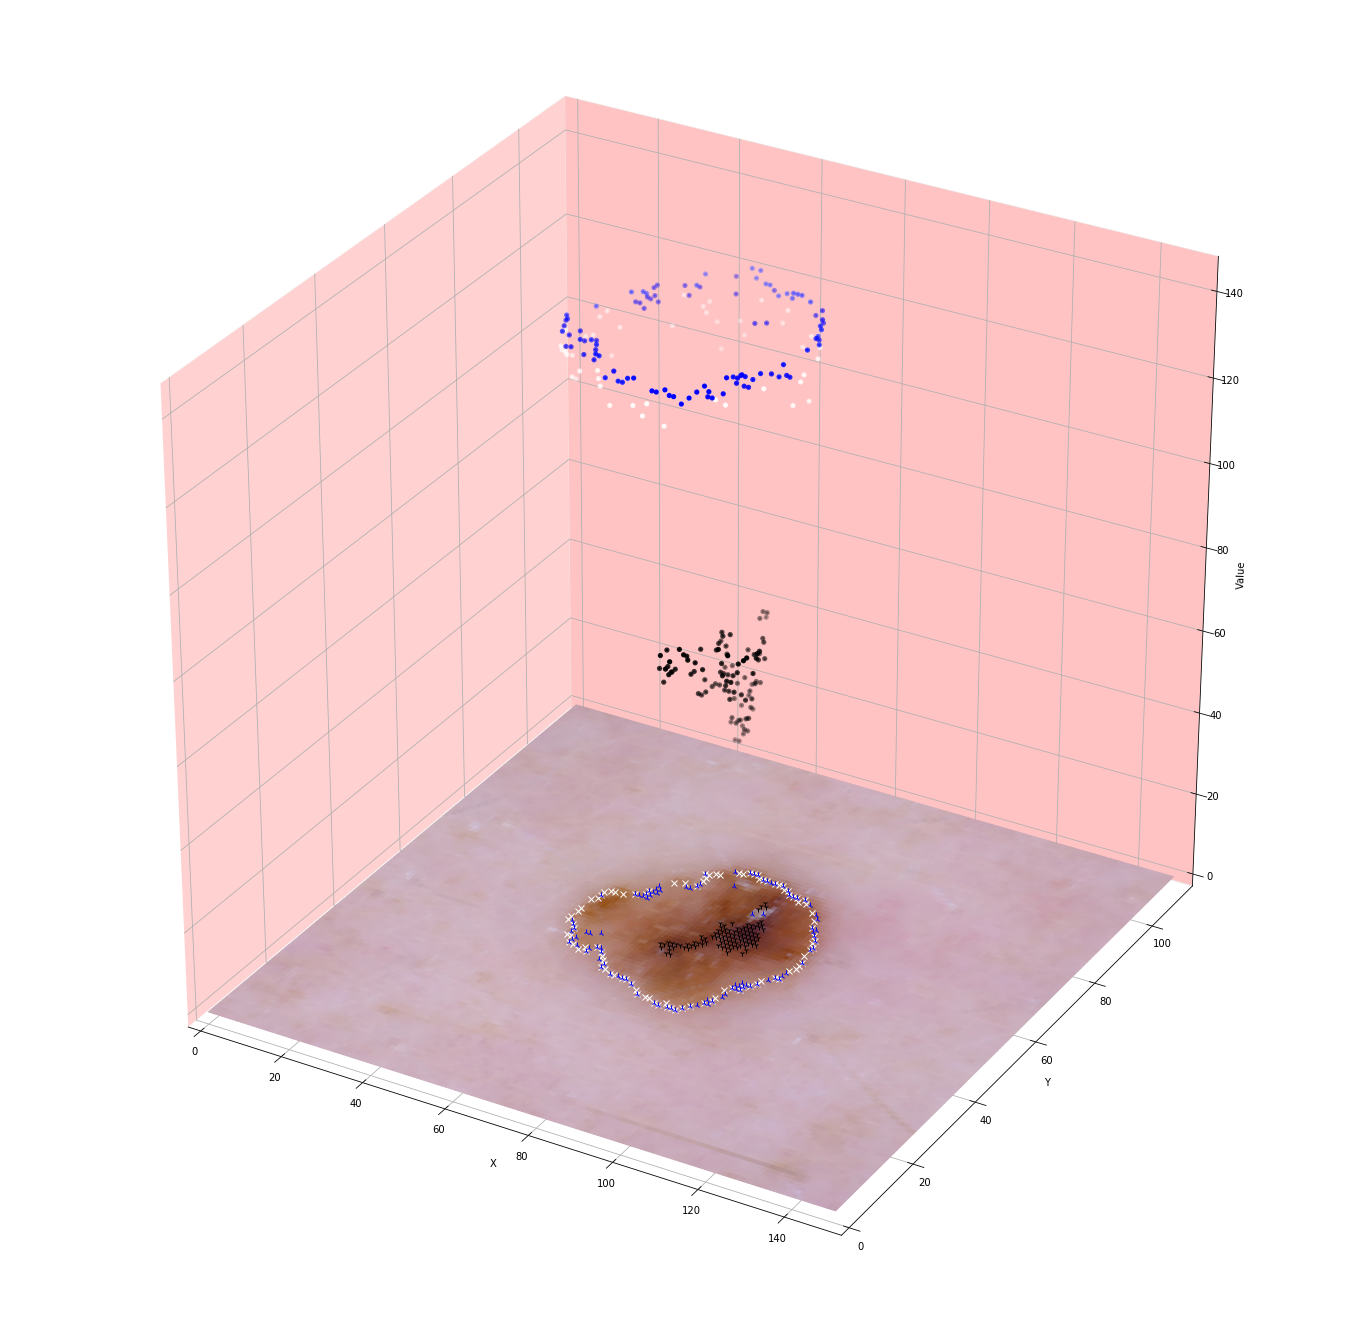
\includegraphics[width=\linewidth]{simple_mel4.png}
  \caption{Grayscale Simple Sampling Method}
\end{subfigure}%
\begin{subfigure}{.5\textwidth}
  \centering
  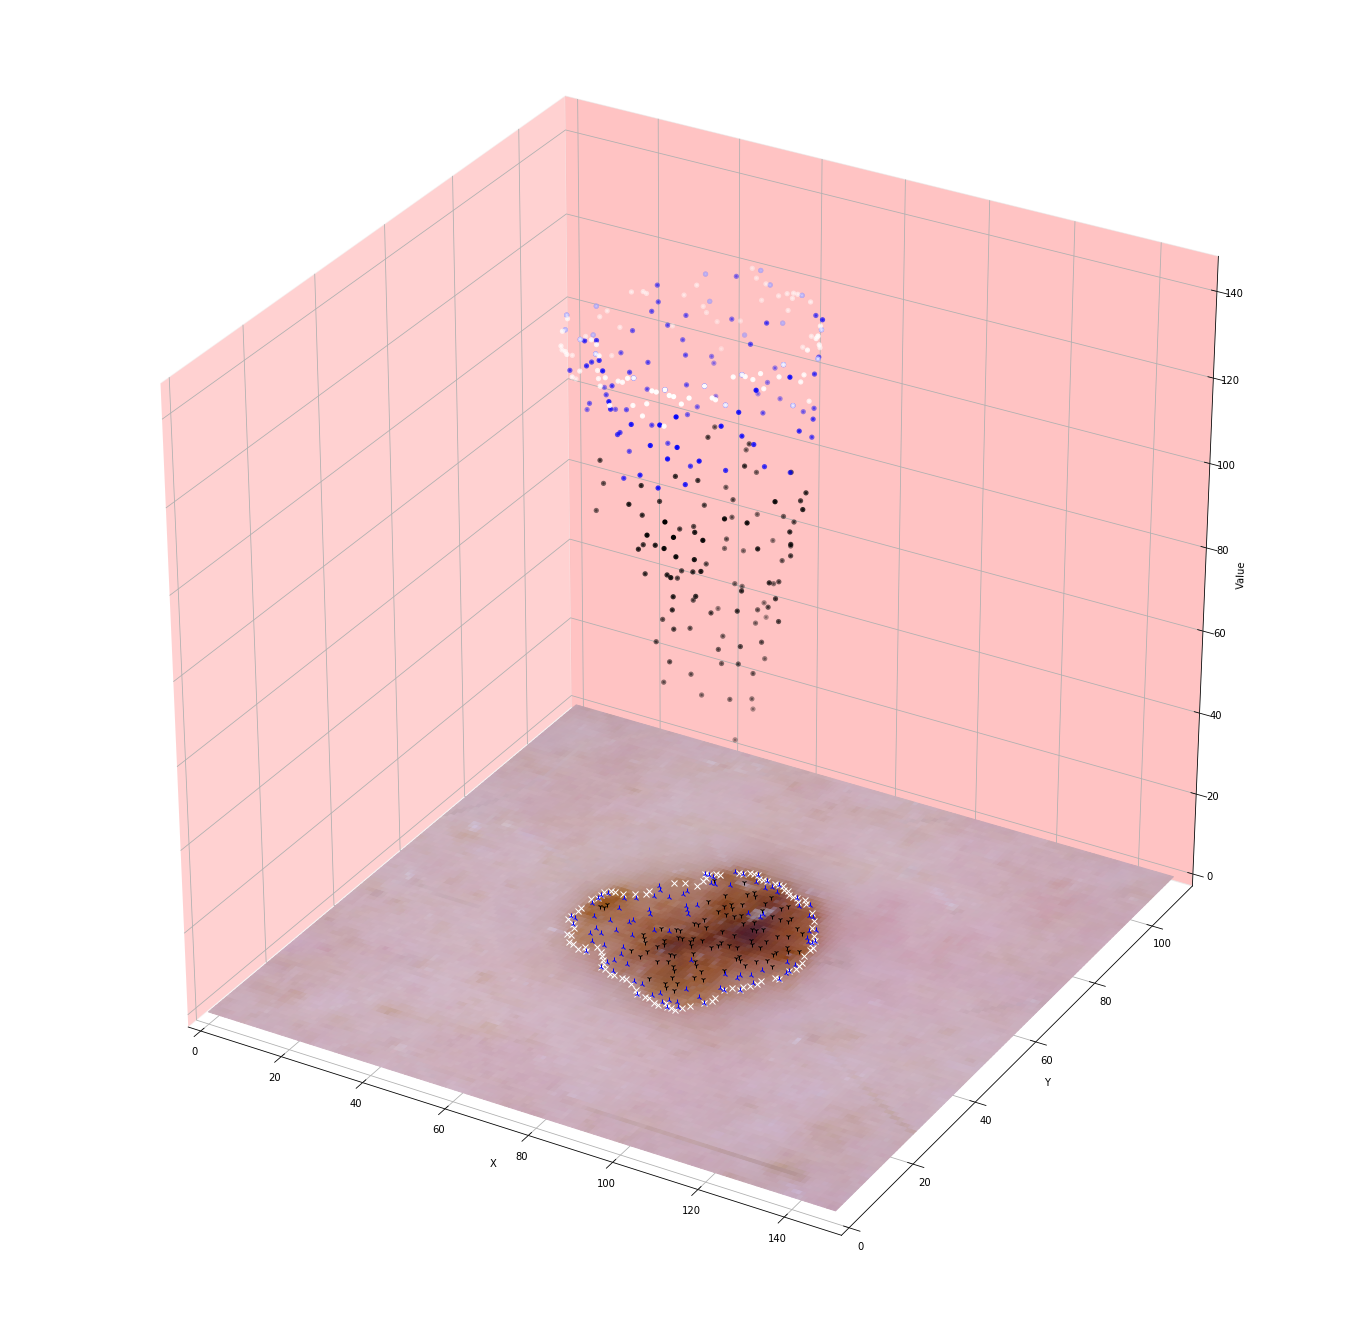
\includegraphics[width=\linewidth]{cluster_mel4.png}
  \caption{Grayscale Cluster Sampling Method}
\end{subfigure}
\caption{{\bfseries MEL Image:} 100 boundary (white), 100 lightest interior (blue), and 100 darkest interior (black) pixels}
\label{fig:mel}
\end{figure}

\begin{figure}
\centering
\begin{subfigure}{.5\textwidth}
  \centering
  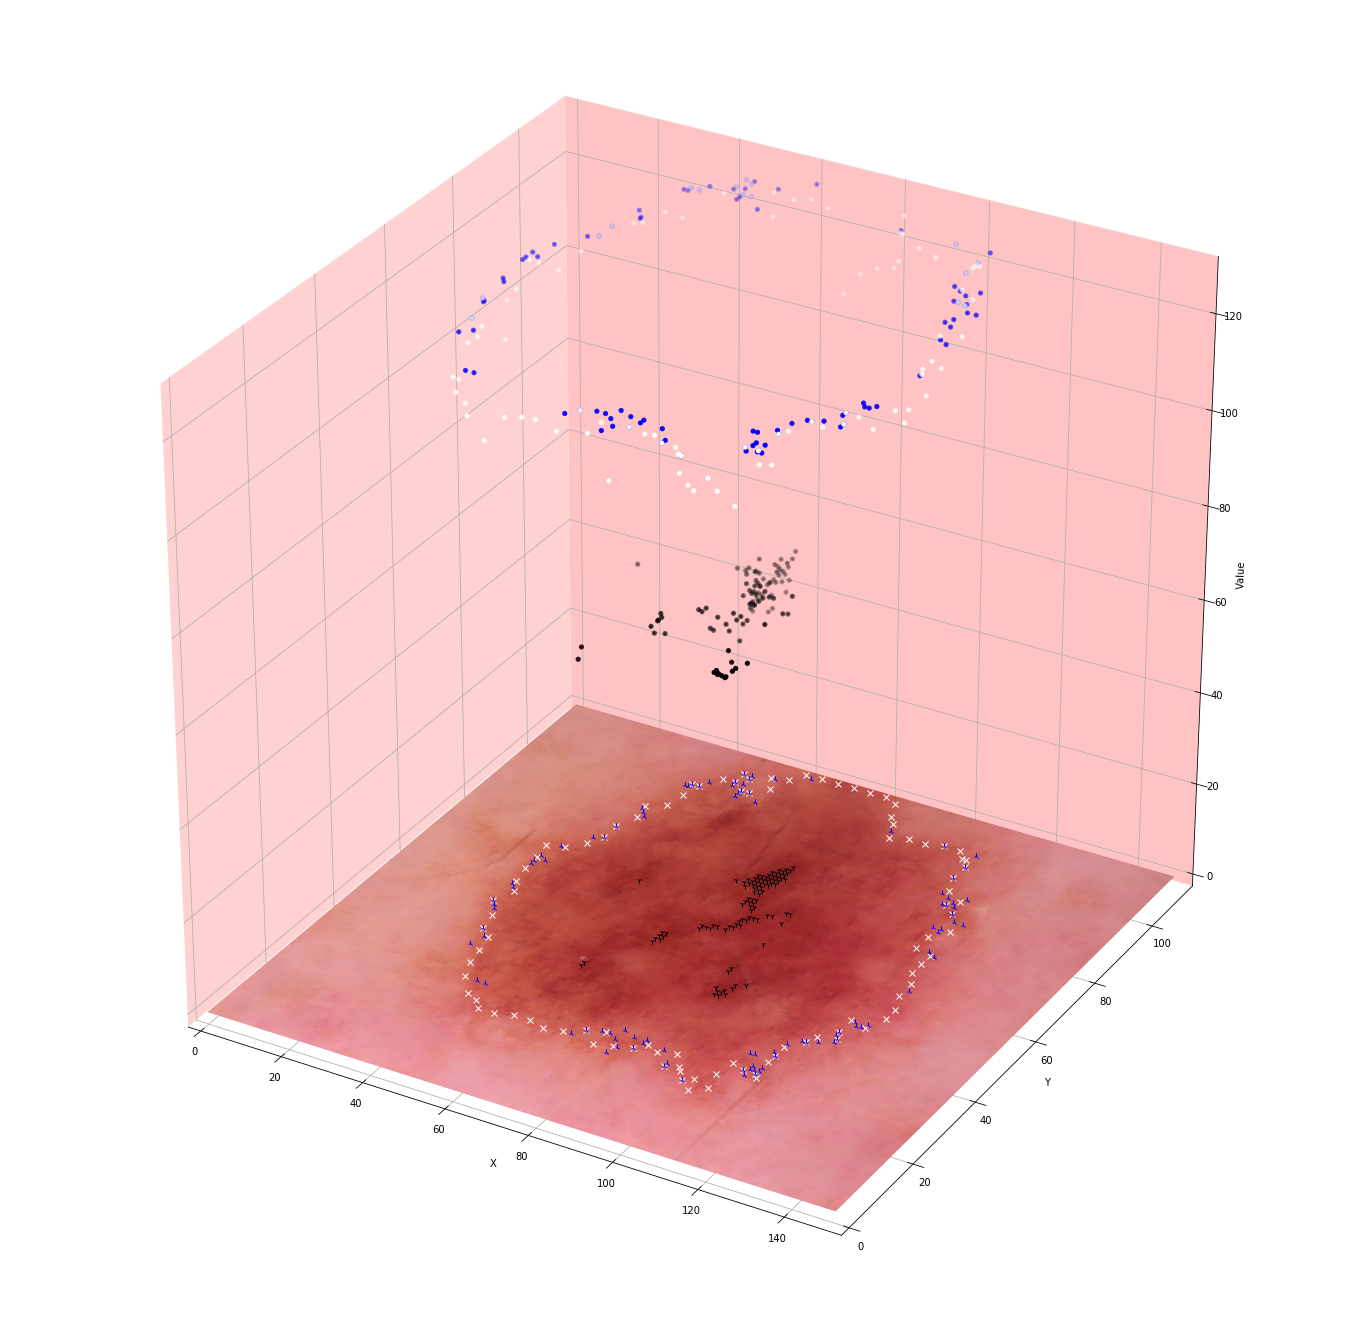
\includegraphics[width=\linewidth]{simple_nv20.png}
  \caption{Grayscale Simple Sampling Method}
\end{subfigure}%
\begin{subfigure}{.5\textwidth}
  \centering
  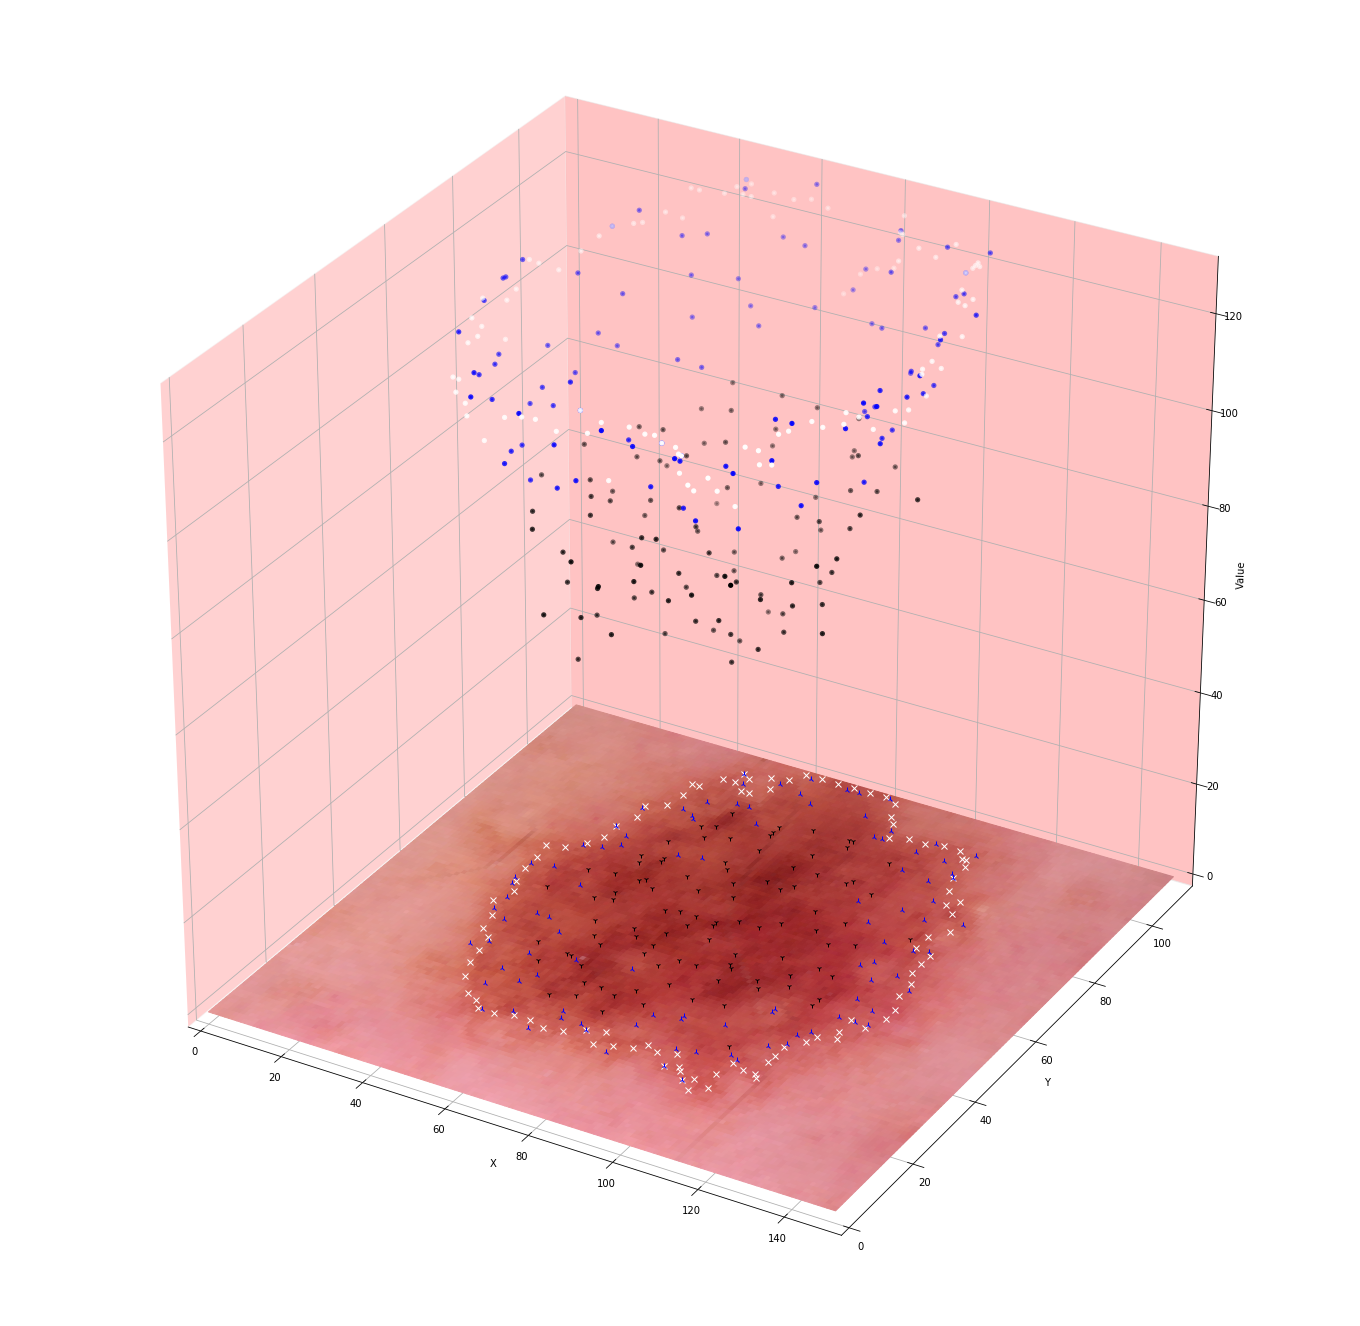
\includegraphics[width=\linewidth]{cluster_nv20.png}
  \caption{Grayscale Cluster Sampling Method}
\end{subfigure}
\caption{{\bfseries NV Image:} 100 boundary (white), 100 lightest interior (blue), and 100 darkest interior (black) pixels}
\label{fig:nv}
\end{figure}

One notable drawback to the cluster sampling method is that many of the point clouds resulting from the cluster sampling method end up looking extremely similar which ultimately resulted in poorer performance during the classification process. As a result, we determined that it would be best to use the simple sampling method for classifying the various types of skin cancer. 

After the point clouds were sampled for each image, the pixel locations and intensities were saved to a .csv file so that they could be reloaded and processed in the topological data analysis phase of the preprocessing pipeline.

\subsection{Computing Death Vectors and Persistence Landscapes}

This step of the data preprocessing pipeline was implemented in RStudio using a script provided by Dr. Bubenik that we coded during the semester with the \href{https://cran.r-project.org/web/packages/TDA/index.html}{TDA Package}. Since the point clouds used were generated in the previous step, we first loaded the point cloud data from the saved .csv files. The pipeline in R was as follows:
\begin{enumerate}
    \item For each image, we used the sampled 100 boundary points and the 100 darkest points from the simple sampling method for a total of 200 points per image
    \item We used the Vietoris-Rips complex in the TDA pipeline to determine the death vector and persistence landscape for the sampled point cloud from each image
\end{enumerate}

After processing the sampled data in R, for each image we had
\begin{itemize}
    \item One death vector of length 199
    \item One persistence landscape vector of length 30100
\end{itemize}
The death vectors and persistence landscape vectors were then saved to a .csv file so that they could be reloaded later without having to rerun the TDA data preprocessing code. 

\section{Data Visualization and Classification}

%Following the computation of the death vectors and persistence landscape vectors, we visualized them using principal component analysis and used them as feature vectors to perform classification with support vector machines and deep neural networks.

\subsection{Principal Component Analysis}

As the resulting death vectors and persistence landscape vectors were high dimensional, we performed a principal component analysis to visualize the data in two dimensions. Below we provide two visualizations for both the death vectors and persistence landscape vectors. 
\begin{figure}[H]
\centering
\begin{subfigure}{.5\textwidth}
  \centering
  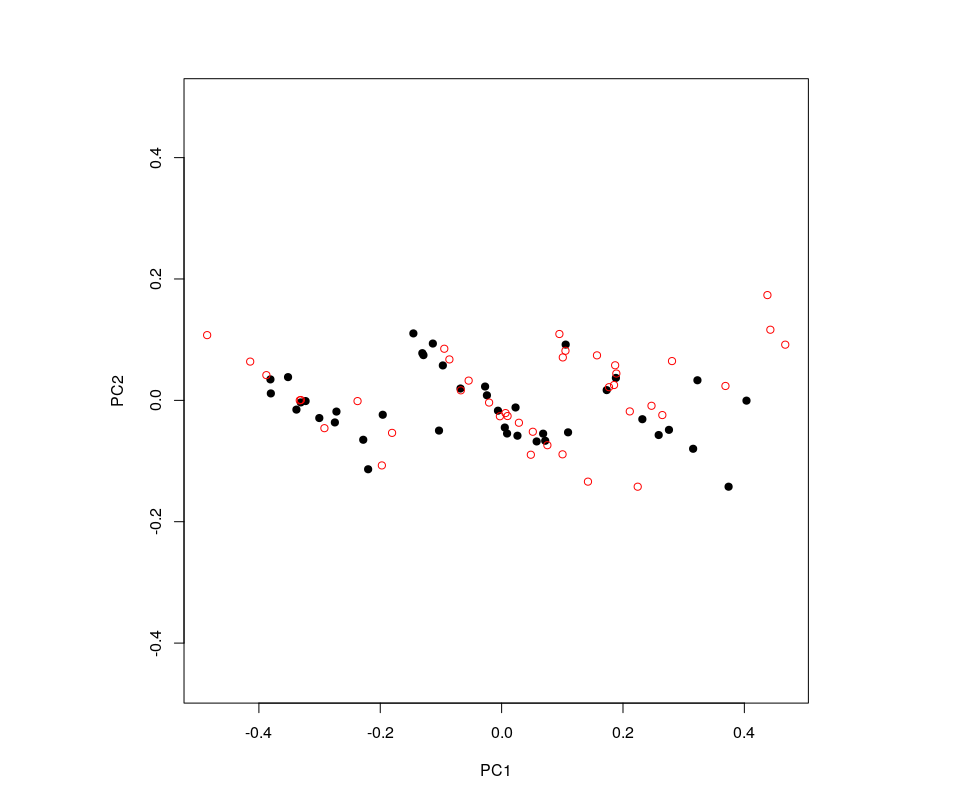
\includegraphics[width=0.9\linewidth]{nv_mel_DV_PCA_Points_Plot.png}
  \caption{Projection of Persistence Landscapes onto\\two leading PCA basis vectors}
\end{subfigure}%
\begin{subfigure}{.5\textwidth}
  \centering
  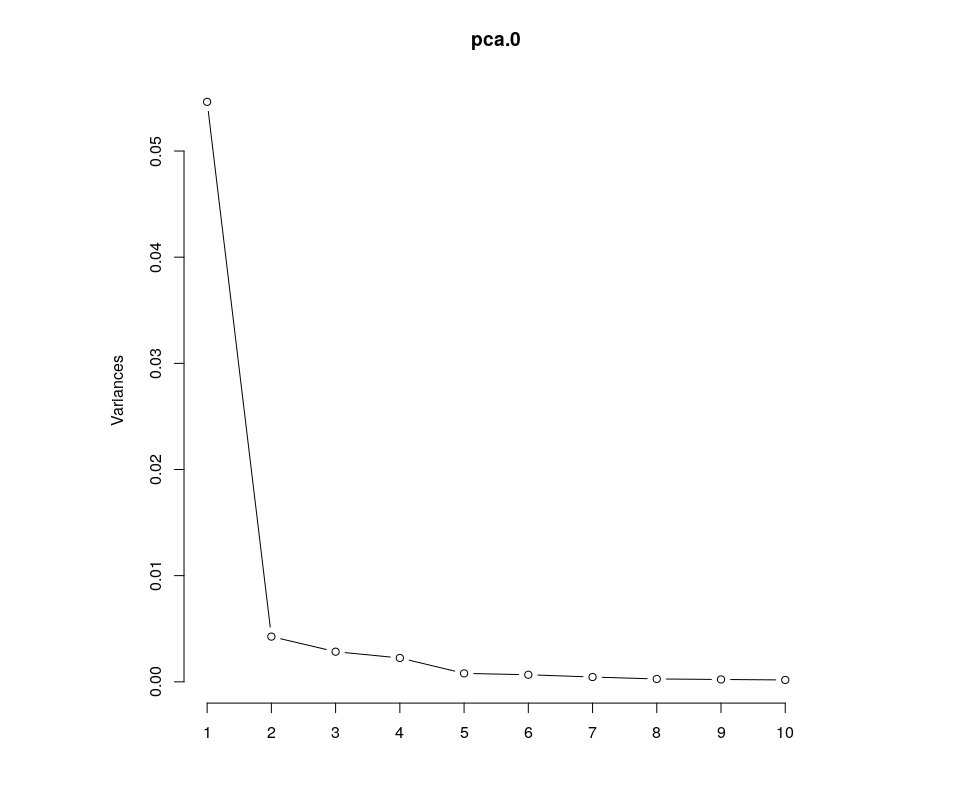
\includegraphics[width=0.9\linewidth]{nv_mel_DV_PCA_Vietoris_Rips.png}
  \caption{Variance in direction of first ten basis vectors from PCA}
\end{subfigure}
\caption{Principal Component Analysis for Death Vectors}
\label{fig:PCA_DV}
\end{figure}
In Figures~\ref{fig:PCA_DV} (A) and \ref{fig:PCA_PL} (A), the points are plotted so that the two different classes, MEL and NV, can be seen as the filled in and hollow points. Using this visualization, it is evident that the two classes are not linearly separable for the death vectors. Some more separation between the two classes is present in the persistence landscape representation. Figures~\ref{fig:PCA_DV} (B) and \ref{fig:PCA_PL} (B) serve to illustrate the variance in the 10 principal components.
\begin{figure}
\centering
\begin{subfigure}{.5\textwidth}
  \centering
  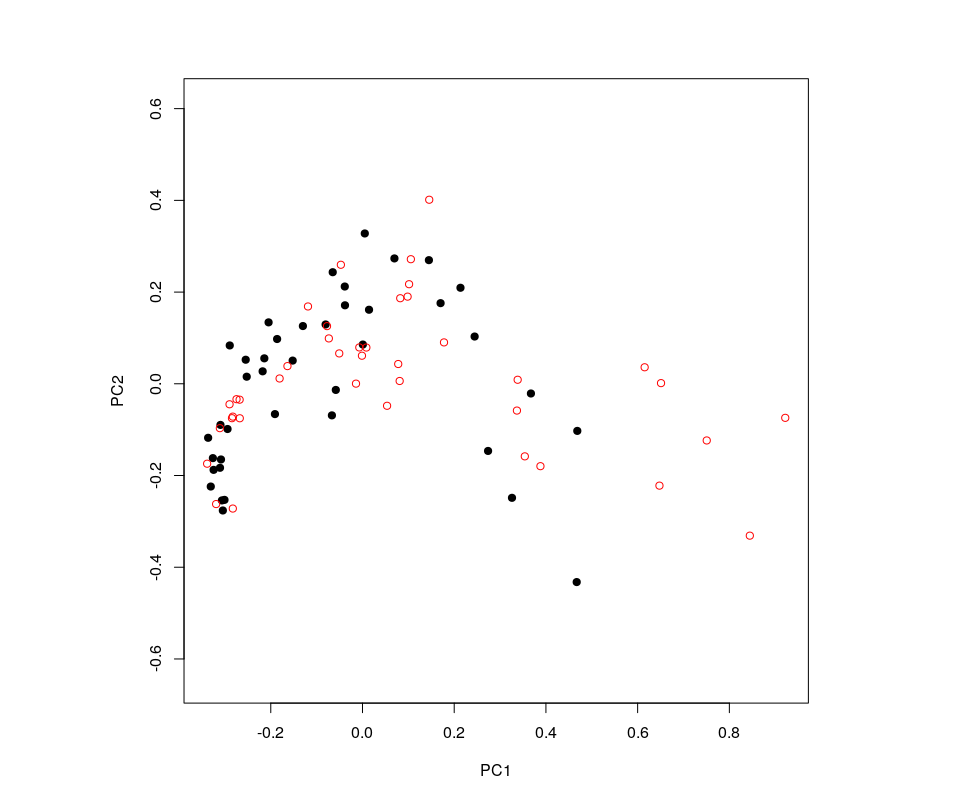
\includegraphics[width=\linewidth]{nv_mel_PL_PCA_Points_Plot.png}
  \caption{Projection of Persistence Landscapes onto\\two leading PCA basis vectors}
\end{subfigure}%
\begin{subfigure}{.5\textwidth}
  \centering
  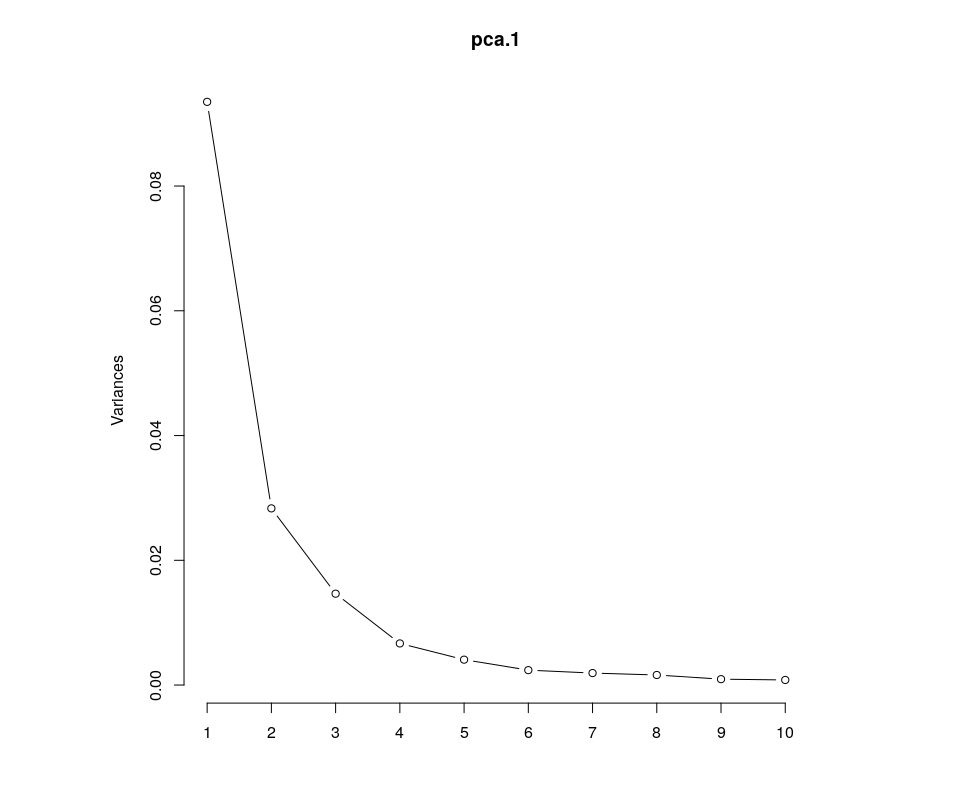
\includegraphics[width=\linewidth]{nv_mel_PL_PCA_Vietoris_Rips.png}
  \caption{Variance in direction of first ten basis vectors from PCA}
\end{subfigure}
\caption{Principal Component Analysis for Persistence Landscape Vectors}
\label{fig:PCA_PL}
\end{figure}

\subsection{Support Vector Machine Classifier}

Based on the principal component analysis visualization, a linear support vector machine would not work well to classify the skin cancer as MEL or NV due to the fact that the classes were not linearly separable in the visualization. As a result, we elected to use a kernel support vector machine classifier with a radial basis function (RBF) kernel. We determined two kernel SVMs:
\begin{enumerate}
    \item RBF SVM using Death Vectors
    \item RBF SVM using Persistence Landscape Vectors
\end{enumerate}
To compute the SVMs we used the \href{https://www.rdocumentation.org/packages/kernlab/versions/0.9-29/topics/ksvm}{R package ksvm} with the kernel set equal to {\bfseries rbfdot}. We used an 80/20 training/testing split so that the training set consisted of 64 images and the validation set consisted of 16 images. 
\begin{figure}[H]
\centering
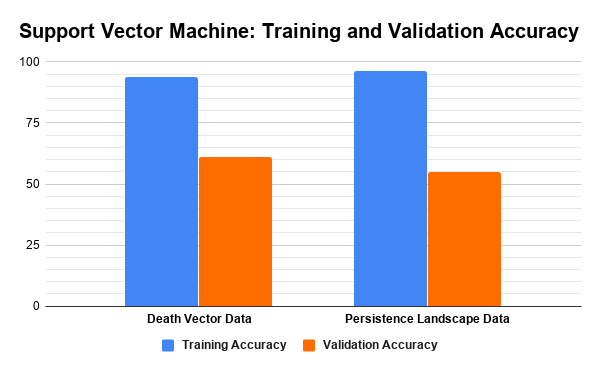
\includegraphics[width=0.5\textwidth]{SVM-Graph.png}
\caption{Training and Validation Accuracy for Death Vector and Persistence Landscape Vector SVMs}
\label{fig:SVM}
\end{figure}
In Figure~\ref{fig:SVM}, the training and validation accuracy for each SVM are plotted in a bar graph. As evident from Figure \ref{fig:SVM}, the large difference between the training and validation accuracy for each model indicates that the SVM classifiers are suffering from overfitting. Based on this issue, we decided to use a deep neural network to perform classification.

\subsection{Deep Neural Network Classifier}

Based on the fact that the SVMs classifiers were suffering from overfitting, we elected to use neural networks as an alternative method to classify the MEL and NV images. We implemented two deep neural networks:
\begin{enumerate}
    \item Deep Neural Network using Death Vectors as Feature Vectors
    \item Deep Neural Network using Persistence Landscape Vectors as Feature Vectors
\end{enumerate} 
To model and train the neural networks we used the Python packages \href{https://www.tensorflow.org/}{TensorFlow} and \href{https://keras.io/}{Keras}. We used \href{https://colab.research.google.com/notebooks/welcome.ipynb#recent=true}{Google Colab} with a GPU accelerator to reduce the training time of the deep neural networks. As in the training of the SVM classifiers, we used an 80/20 training/testing split so that the training set consisted of 64 images and the validation set consisted of 16 images. 

The network topologies varied for the neural network depending on the features used for classification. For both networks we used ReLU activation functions. We used dropout layers after each activation layer to avoid overfitting of the trained networks. Additionally, we used batch normalization to reduce the amount of time required to train each network. Summaries of the topologies of the neural network using the death vectors and persistence landscape vectors are provided in Figure~\ref{fig:DNN_Summary}.
\begin{figure}[H]
\centering
\begin{subfigure}{.5\textwidth}
  \centering
  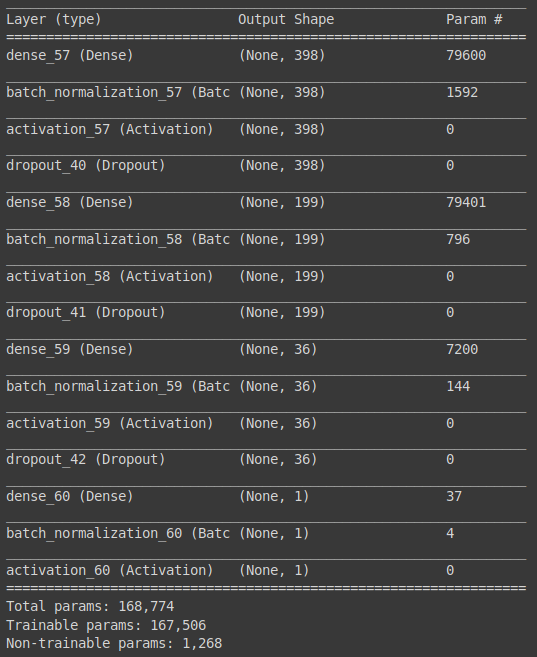
\includegraphics[width=0.8\linewidth]{DV_DNN_Summary.png}
  \caption{DNN using Death Vectors}
\end{subfigure}%
\begin{subfigure}{.5\textwidth}
  \centering
  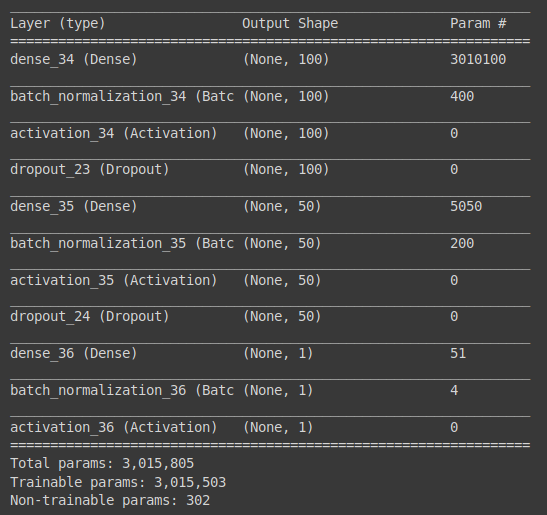
\includegraphics[width=0.8\linewidth]{PL_DNN_Summary.png}
  \caption{DNN using Persistence Landscape Vectors}
\end{subfigure}
\caption{Summary of Deep Neural Network Topologies for Classification}
\label{fig:DNN_Summary}
\end{figure}
\noindent Due to the large size of the persistence landscape vectors, we were unable to scale up the number of input and hidden neurons for the deep neural network that used the persistence landscape vectors as we were encountering poor training improvements and occasional memory issues. Ideally, we would have been able to greatly increase the number of input and hidden neurons in this network.

We trained the deep neural network using the death vectors for a total of 120 epochs with a batch size of $5$. We used the \href{https://www.tensorflow.org/api_docs/python/tf/keras/optimizers/Adam}{Adam optimizer} with an initial learning rate of \texttt{1e-4} and implemented a callback to reduce the learning rate when the validation loss became stagnant. The deep neural network using the persistence landscape vectors was trained for a total of 150 epochs with a batch size of $8$. As in the previous network, we also used the \href{https://www.tensorflow.org/api_docs/python/tf/keras/optimizers/Adam}{Adam optimizer} and implemented a callback to reduce the learning rate when the validation loss became stagnant, however, we started with an initial learning rate of \texttt{1e-2}. The training and validation accuracy for the two deep neural networks are provided in Figure~\ref{fig:DNN_acc}. As observed by the figure, neither of the deep neural network classifiers suffer from overfitting and both achieve much better validation accuracy than the SVM classifiers.

\begin{figure}[H]
\centering
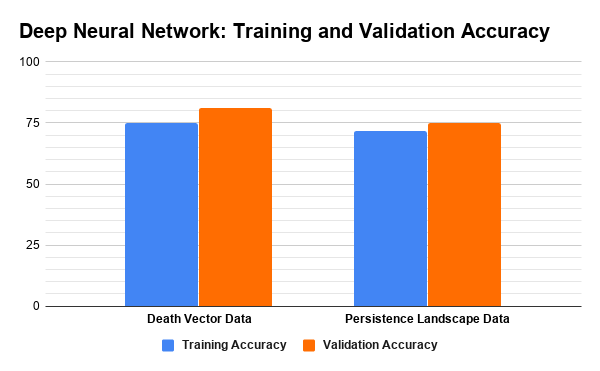
\includegraphics[width=0.5\textwidth]{DNN-Graph.png}
\caption{Training and Validation Accuracy for Death Vector and Persistence Landscape Vector Deep Neural Networks}
\label{fig:DNN_acc}
\end{figure}

\section{Conclusion and Future Work}

In this project we successfully modeled and trained a classifier for MEL and NV images that does not suffer from overfitting and achieves an accuracy of $81.25\%$ on the validation data set. However, we should note that this was only achieved on a very small subset of the data and we believe that better performance can be achieved by making the following improvements:
\begin{itemize}
    \item {\bfseries Update the Sampling Method}: We developed our own method for sampling the points from each of the skin cancer images but we believe that this could be improved by:
    \begin{enumerate}
        \item[(a)] Using the winning boundary detection method developed for the ISIC 2018 challenge to sample points from the boundary of the skin cancer in each image
        \item[(b)] Refining the sampling method used to sample points from the interior of the skin cancer in each image. One idea may include using \href{https://scikit-learn.org/stable/modules/generated/sklearn.cluster.DBSCAN.html}{DBSCAN} to identify density clusters in the interior of the skin cancer then stratified sampling across the clusters to get a uniform number of points sampled in each image.
    \end{enumerate} 
    \item {\bfseries Streamline Data Preprocessing Pipeline}: Figure out how to use the \href{https://pypi.org/project/scikit-tda/}{scikit-tda} package so that the topological data analysis can be performed in Python to reduce the movement from Python to R back to Python
    \item {\bfseries Use More Data}: Now that a data preprocessing pipeline has been established and tested, once it is further refined more images and more classes should be sampled from to create a larger data set of death vectors and persistence landscapes
    \item {\bfseries Multiclass Classification}: Once all of the data has be transformed to death vectors and persistence landscapes, we would like to attempt multiclass classification using deep neural networks to see what accuracy can be achieved.
\end{itemize}

%% ------------------- Bibliography -------------------- %%
\bibliographystyle{unsrt}
\bibliography{machine-learning}

\end{document}